\chapter{El Mundo Real: Problemas Físicos No Lineales}
\label{chap:nonlinear}

%==================================================================================
\section{Abrazando la Complejidad del Mundo Real}
%==================================================================================

En los Capítulos~\ref{chap:poisson} y \ref{chap:heat}, construimos una base sólida para resolver problemas de conducción de calor. Sin embargo, lo hicimos bajo una suposición simplificadora crucial: que las propiedades del material (\(k, \rho, c_p\)) eran constantes. En el mundo real, esta rara vez es la situación.

Este capítulo aborda el siguiente nivel de realismo físico: los \textbf{problemas no lineales}. Un problema se vuelve no lineal cuando las propiedades que gobiernan su comportamiento dependen de la propia solución que buscamos. Para la Ecuación del Calor, esto ocurre comúnmente cuando la conductividad térmica depende de la temperatura, \(k = k(T)\).

Resolver este tipo de problemas requiere un salto conceptual y matemático. Ya no podemos ensamblar una única matriz y resolver un sistema de ecuaciones lineales. Debemos adoptar un enfoque \textbf{iterativo}. Presentaremos el \textbf{Método de Newton-Raphson}, un algoritmo poderoso y universal que forma la columna vertebral de la mayoría de los solvers de elementos finitos para problemas no lineales.

\begin{center}
\begin{tabular}{|p{0.9\textwidth}|}
\hline
\textbf{CONTEXTO INGENIERIL} \\
La no linealidad es la norma, no la excepción, en la ingeniería de vanguardia. Consideremos:
\begin{itemize}
    \item \textbf{Procesamiento de Materiales:} En tratamientos térmicos de aceros, la conductividad térmica y la capacidad calorífica varían drásticamente con la temperatura, afectando la velocidad de enfriamiento y las propiedades finales del material.
    \item \textbf{Electrónica de Potencia:} La resistividad del silicio en un semiconductor cambia con la temperatura. A medida que se calienta por el paso de corriente, su capacidad para disipar ese calor también cambia, un acoplamiento no lineal crítico.
    \item \textbf{Ablación Térmica:} En escudos térmicos para reentrada atmosférica, las propiedades del material cambian a temperaturas extremas, un comportamiento altamente no lineal que determina la supervivencia del vehículo.
\end{itemize}
Dominar los métodos no lineales nos permite simular la física con una fidelidad mucho mayor. \\
\hline
\end{tabular}
\end{center}

%==================================================================================
\section{El Origen de la No Linealidad en la Ecuación del Calor}
\label{sec:nonlinear-origin}
%==================================================================================
Recordemos la forma fuerte transitoria de la Ecuación del Calor de la Ecuación~\eqref{eq:heat-strong-form}:
\[
    \rho c_p \frac{\partial T}{\partial t} - \nabla \cdot (k \nabla T) = f
\]
Hasta ahora, hemos tratado a \(k\) como una constante. Sin embargo, para la mayoría de los materiales, la conductividad es función de la temperatura. Una aproximación común es una relación lineal:
\begin{equation}
    k(T) = k_0 (1 + \alpha (T - T_{\text{ref}}))
    \label{eq:k_of_T}
\end{equation}
donde \(k_0\) es la conductividad a una temperatura de referencia \(T_{\text{ref}}\) y \(\alpha\) es un coeficiente del material.

Cuando sustituimos \(k(T)\) en la Ecuación del Calor, el término de difusión se convierte en \(\nabla \cdot (k(T) \nabla T)\). Este término es ahora \textbf{no lineal} porque el coeficiente \(k(T)\) que multiplica a la derivada de la solución (\(\nabla T\)) depende de la propia solución (\(T\)).

%==================================================================================
\section{El Enfoque Iterativo: El Método de Newton}
\label{sec:newton-method}
%==================================================================================

%----------------------------------------------------------------------------------
\subsection{Por Qué Fracasa el Enfoque Lineal}
%----------------------------------------------------------------------------------
En los capítulos anteriores, nuestro procedimiento variacional nos llevaba a un sistema de ecuaciones algebraicas de la forma \(\mathbf{A}\mathbf{T}^n = \mathbf{b}\). La clave era que la ``matriz del sistema'' \(\mathbf{A}\) era constante: dependía únicamente de la malla y de las propiedades del material (que asumimos constantes). Podíamos ensamblarla una vez y resolver el sistema.

Cuando \(k=k(T)\), la matriz del sistema ahora depende de la solución que estamos tratando de encontrar: \(\mathbf{A}(T^n)\mathbf{T}^n = \mathbf{b}\). Esto rompe completamente el paradigma anterior. No podemos construir la matriz sin conocer la solución, y no podemos encontrar la solución sin tener la matriz. Es un problema circular que exige un nuevo enfoque.

%----------------------------------------------------------------------------------
\subsection{La Estrategia de Newton: Linealizar para Conquistar}
%----------------------------------------------------------------------------------
El Método de Newton es una técnica para encontrar las raíces de un sistema de funciones no lineales. Su idea central, adaptada a nuestro contexto, es un proceso iterativo:
\begin{enumerate}
    \item Partir de una \textbf{suposición inicial} para la solución en el paso de tiempo actual, \(T_k^n\) (donde \(k\) es el contador de la iteración de Newton). Una buena suposición es la solución del paso de tiempo anterior, \(T^{n-1}\).
    \item \textbf{Linealizar} el problema en torno a esa suposición. Esto es análogo a aproximar una curva compleja por su línea tangente en un punto.
    \item Resolver este problema \textit{lineal} aproximado para encontrar una \textbf{corrección}, \(\delta T\).
    \item \textbf{Actualizar} la suposición con la corrección: \(T_{k+1}^n = T_k^n + \delta T\).
    \item \textbf{Repetir} los pasos 2-4 hasta que la corrección \(\delta T\) sea suficientemente pequeña, indicando que la solución ha convergido.
\end{enumerate}

%----------------------------------------------------------------------------------
\subsection{Aplicando Newton a Nuestra Forma Débil}
%----------------------------------------------------------------------------------
Para implementar el método de Newton, primero reescribimos nuestra forma débil como un \textbf{residuo} \(F(T^n; v)\) que debe ser cero. A partir de la forma débil transitoria, Ecuación~\eqref{eq:heat-weak}, y moviendo todos los términos al lado izquierdo, el residuo para el paso de tiempo \(n\) es:
\begin{equation}
    F(T^n; v) = \int_{\Omega} \left( \rho c_p (T^n - T^{n-1}) v + \Delta t \, k(T^n) \nabla T^n \cdot \nabla v \right) dV - \int_{\Omega} \Delta t \, f^n v \, dV = 0
    \label{eq:nonlinear-residual}
\end{equation}
El método de Newton busca iterativamente una solución \(T^n\) que anule este residuo para toda función de prueba \(v\). Para ello, se debe calcular la derivada del residuo con respecto a la solución, una cantidad llamada el \textbf{Jacobiano}, \(J\). Aunque su derivación matemática es compleja (ver, por ejemplo, \cite{Elman2014}), su significado es crucial: nos dice cómo un pequeño cambio en la solución, \(\delta T\), afecta al residuo.

Afortunadamente, \fenics calcula este complejo Jacobiano \textbf{automáticamente}. Solo necesitamos proporcionarle la forma del residuo no lineal, y él se encarga del resto. En cada iteración de Newton, \fenics resuelve el siguiente problema \textit{lineal} para la corrección \(\delta T\):

\begin{center}
\fbox{\begin{minipage}{0.9\textwidth}
\textbf{Problema Lineal a Resolver en Cada Iteración de Newton} \\
Dada una solución tentativa \(T_k^n\), encontrar la corrección \(\delta T\) tal que para todo \(v\):
\begin{equation}
    J(\delta T; v) = -F(T_k^n; v)
    \label{eq:newton-system}
\end{equation}
\end{minipage}}
\end{center}
Una vez resuelto para \(\delta T\), se actualiza la solución y el proceso continúa. Con esta poderosa maquinaria, estamos listos para resolver problemas no lineales.

%==================================================================================
\section{De la Teoría a la Práctica: Implementación No Lineal en \fenics}
\label{sec:nonlinear-fenics}
%==================================================================================
La teoría del método de Newton es elegante, pero la verdadera magia reside en cómo herramientas modernas como \fenics nos permiten implementarla con cambios mínimos en nuestro código. Vamos a aplicar esta maquinaria a un problema clásico de la metalurgia.

%----------------------------------------------------------------------------------
\subsection{Caso de Estudio: Tratamiento Térmico de un Disco de Acero}
%----------------------------------------------------------------------------------
Consideremos un disco de acero inoxidable (ej. AISI 304), inicialmente calentado a una temperatura uniforme de \(800 \, ^\circ\text{C}\). De repente, su borde exterior se expone a un ambiente refrigerado que lo mantiene a \(20 \, ^\circ\text{C}\) (un proceso análogo a un temple o *quenching*). Queremos simular la evolución de la temperatura dentro del disco durante los primeros 60 segundos.

La clave de este problema es que la conductividad térmica del acero inoxidable no es constante, sino que depende fuertemente de la temperatura. Usaremos una relación lineal extraída de datos de ingeniería para capturar esta física.

%----------------------------------------------------------------------------------
\subsection{Planteamiento del Problema Numérico}
%----------------------------------------------------------------------------------
Definimos los componentes de nuestra simulación no lineal:
\begin{itemize}
    \item \textbf{Dominio y Geometría (\(\Omega\)):} Un disco 2D de radio \(R = 0.05\) m.
    \item \textbf{Propiedades del Material (Acero AISI 304, aproximadas):}
    \begin{itemize}
        \item \textbf{Conductividad Térmica No Lineal (\(k(T)\)):} \(k(T) = 14.6 + 0.0157 \times T\). La conductividad aumenta con la temperatura.
        \item \textbf{Densidad:} \(\rho = 7900 \, \text{kg/m}^3\).
        \item \textbf{Capacidad Calorífica:} \(c_p = 500 \, \text{J/(kg·K)}\).
    \end{itemize}
    \item \textbf{Fuente de Calor (\(f\)):} No hay fuentes internas, \(f=0\).
    \item \textbf{Condiciones de Contorno (\(\partial\Omega\)):} El borde exterior del disco se mantiene a una temperatura fija: \(T_D = 20 \, ^\circ\text{C}\) (condición de Dirichlet).
    \item \textbf{Condición Inicial:} Al tiempo \(t=0\), todo el disco está a una temperatura uniforme: \(T(x,y,t=0) = 800 \, ^\circ\text{C}\).
    \item \textbf{Parámetros Temporales:} Simularemos 60 segundos con un paso de tiempo de \(\Delta t = 1\) s.
\end{itemize}

%----------------------------------------------------------------------------------
\subsection{Implementación y Análisis de Resultados}
%----------------------------------------------------------------------------------
El Listado de Código~\ref{lst:nonlinear-code} muestra la implementación. El cambio crucial con respecto al Capítulo~\ref{chap:heat} es sutil pero profundo: la conductividad \(k\) ahora se define en función de la solución desconocida \(T\). Al hacer esto, el problema se vuelve no lineal. \fenics detecta esto automáticamente y, en lugar de un solver lineal, invoca internamente el método de Newton en cada paso de tiempo.

\begin{codelisting}[h!]
\begin{minted}[frame=lines,
               framesep=2mm,
               linenos,
               fontsize=\small]{python}
from fenics import *

# 1. Definir parámetros
dt = 1.0           # Paso de tiempo
numSteps = 60      # Número de pasos
rho = 7900         # Densidad
cp = 500           # Capacidad calorífica
T_border = 20.0    # Temperatura del borde
T_initial = 800.0  # Temperatura inicial

# 2. Definir la malla y el espacio funcional
mesh = CircleMesh(Point(0, 0), 0.05, 32)
V = FunctionSpace(mesh, 'P', 1)

# 3. Definir condiciones de contorno e iniciales
def boundary(x, onBoundary):
    return onBoundary
bc = DirichletBC(V, Constant(T_border), boundary)

# T es la solución en el tiempo actual n (desconocida)
T = Function(V) 
# Tn es la solución del paso anterior (n-1)
Tn = Function(V)
Tn.assign(interpolate(Constant(T_initial), V))

# 4. Definir el problema variacional no lineal
v = TestFunction(V)
# LA CLAVE: k depende de la solución desconocida T
k = 14.6 + 0.0157*T 
# Definimos el residuo F de la Ecuación (3.2)
F = rho*cp*(T - Tn)*v*dx + dt*k*dot(grad(T), grad(v))*dx

# 5. Bucle temporal con solver no lineal
vtkfile = File('Figuras/nonlinear_solution.pvd')
for n in range(numSteps):
    # FEniCS detecta que F es no lineal en T y usa Newton
    solve(F == 0, T, bc)
    vtkfile << (T, n * dt)
    Tn.assign(T)
\end{minted}
\caption{Script de FEniCS para resolver la Ecuación del Calor no lineal.}
\label{lst:nonlinear-code}
\end{codelisting}

La Figura~\ref{fig:nonlinear-result} muestra la evolución del enfriamiento.

\begin{figure}[h!]
    \centering
    %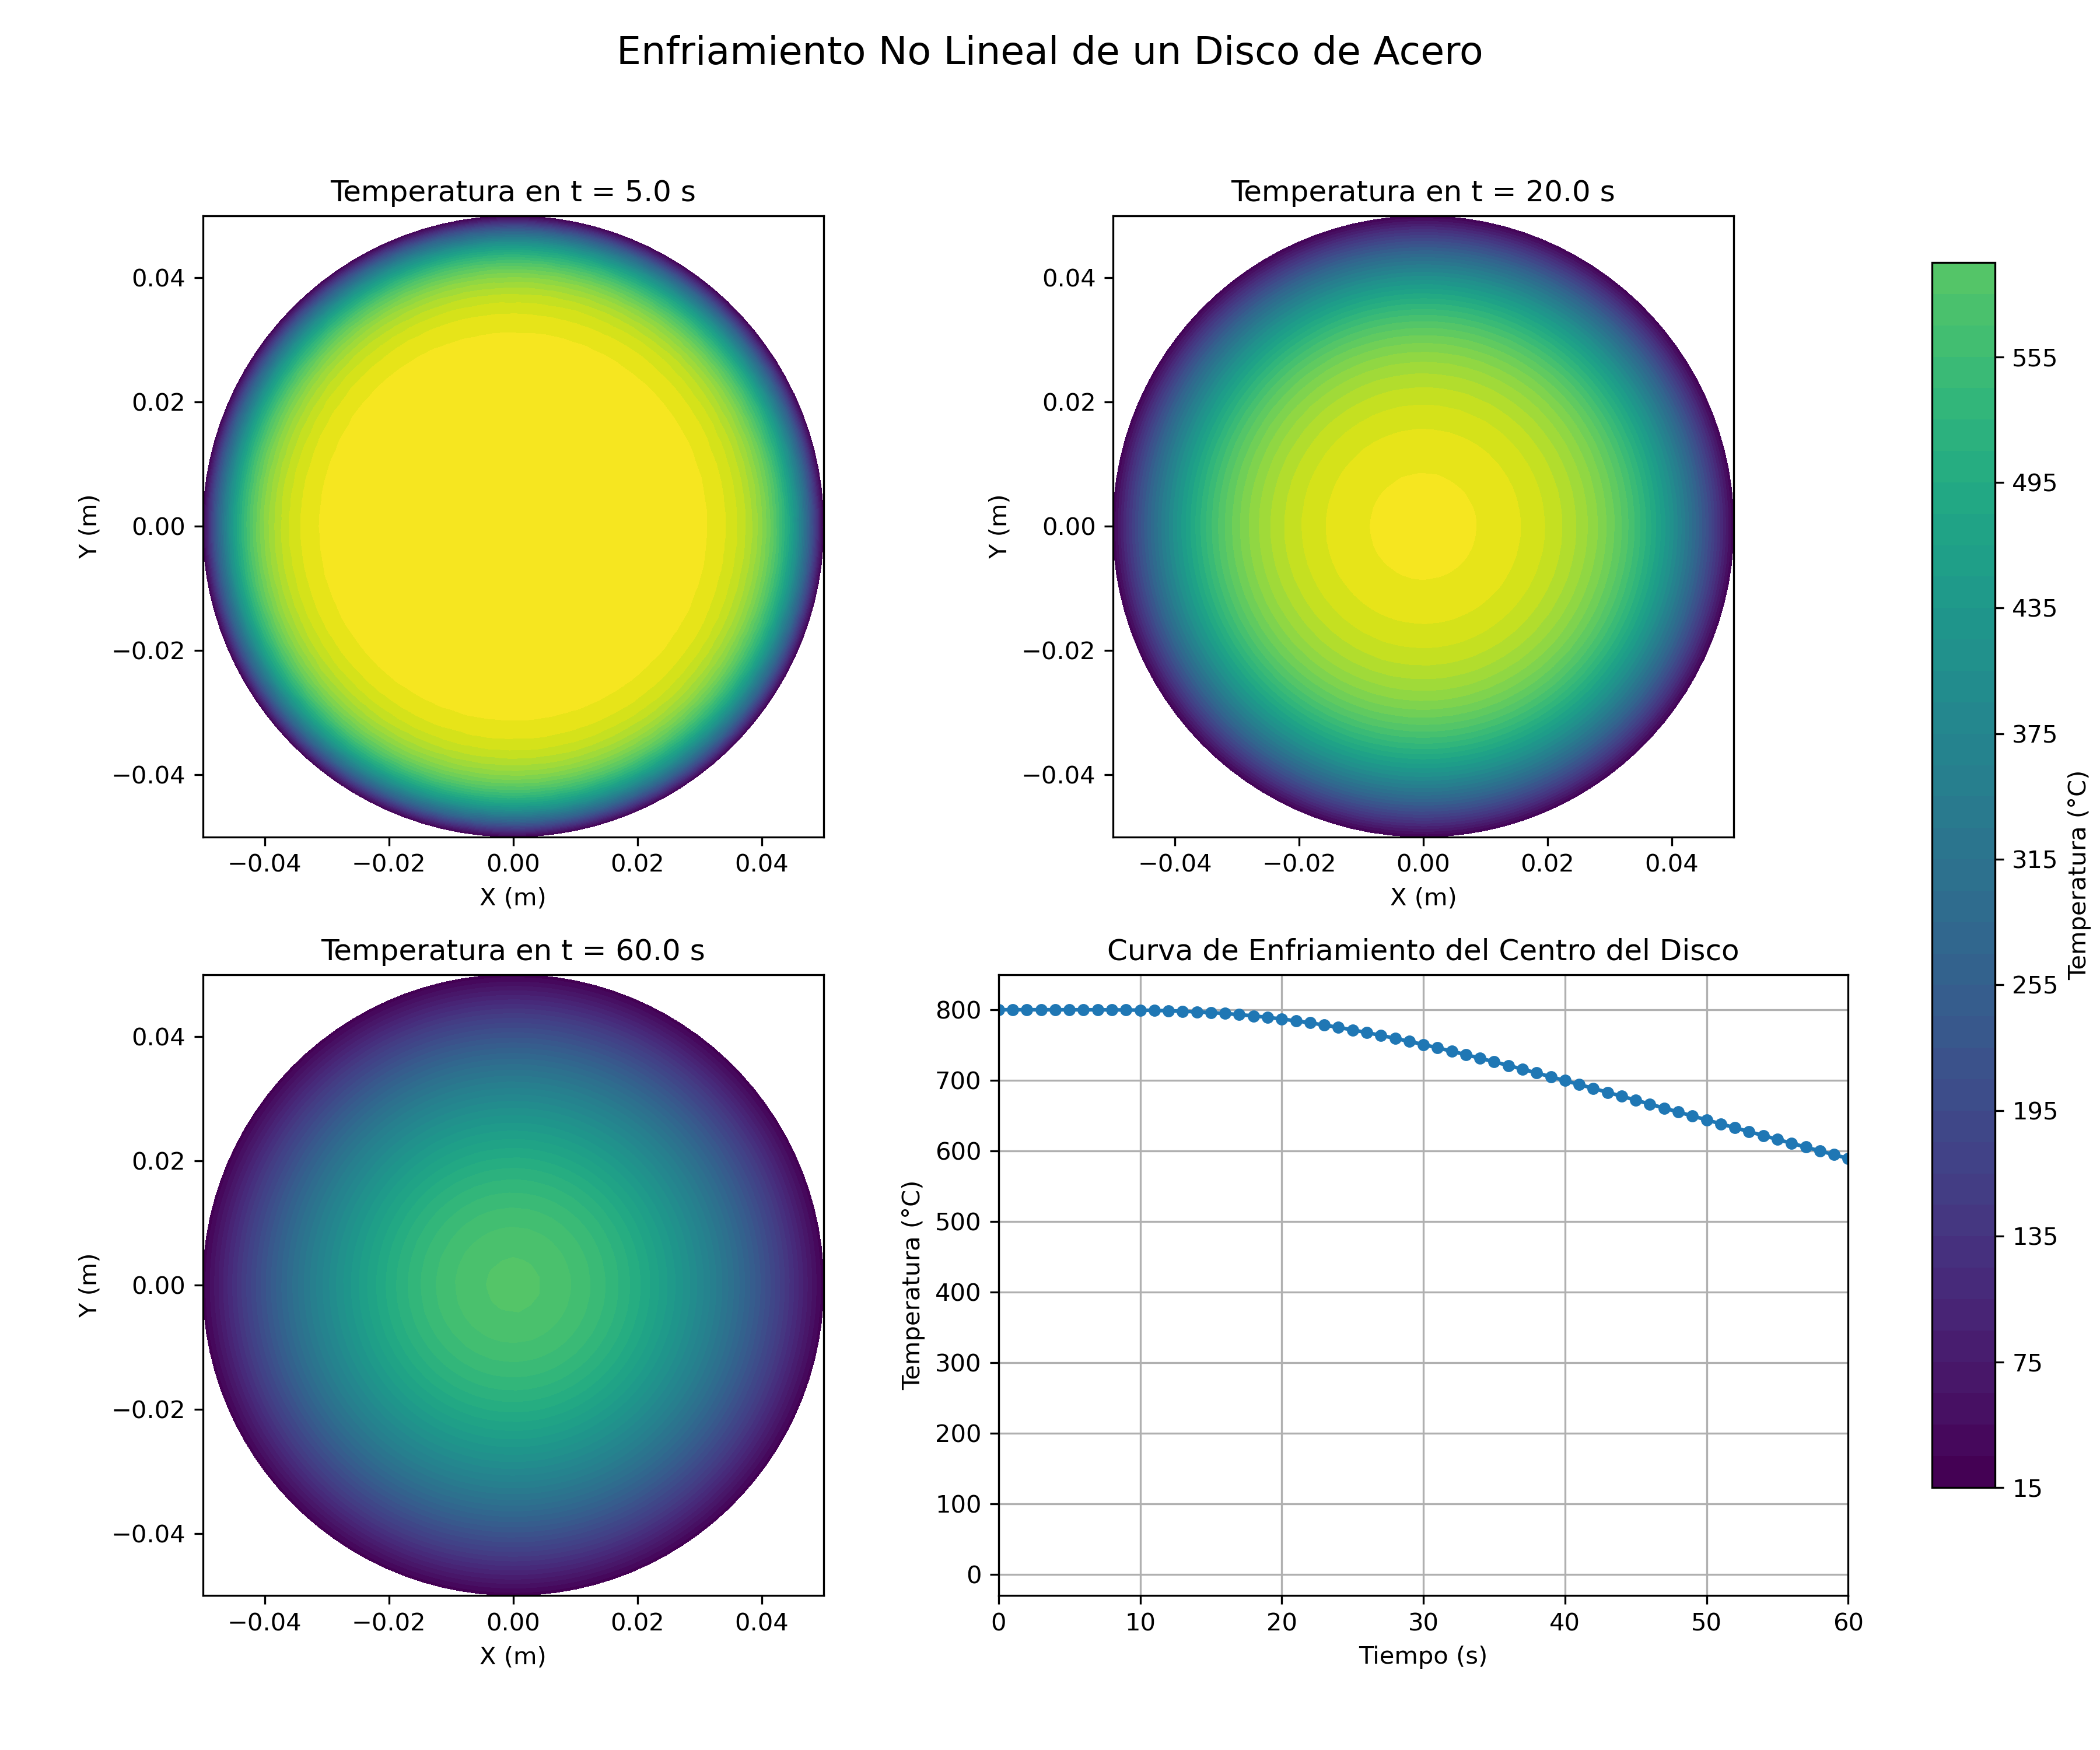
\includegraphics[width=\textwidth]{Figuras/nonlinear_result.png}
    \caption{Narrativa visual del enfriamiento no lineal del disco de acero. Los paneles muestran la rápida caída de temperatura cerca del borde y la difusión más lenta hacia el centro. El gráfico de la derecha muestra la curva de enfriamiento del punto central del disco.}
    \label{fig:nonlinear-result}
\end{figure}

\textbf{Análisis e Impacto Ingenieril:} El resultado clave es la \textit{curva de enfriamiento} (panel derecho). Esta curva no es una simple exponencial, como lo sería en un problema lineal. Al principio, cuando el disco está muy caliente, la conductividad \(k\) es alta, y el calor se extrae eficientemente, provocando una rápida caída de la temperatura. A medida que el disco se enfría, su conductividad disminuye, y la tasa de enfriamiento se reduce.

Este comportamiento es el corazón de la metalurgia. La velocidad a la que se enfría el acero (la pendiente de esta curva) determina su microestructura final (martensita, bainita, etc.) y, por lo tanto, sus propiedades mecánicas como la dureza y la tenacidad. Simular con precisión este proceso no lineal permite a los ingenieros diseñar ciclos de tratamiento térmico para producir aceros con propiedades a medida, una capacidad de un valor industrial inmenso.

%==================================================================================
\section*{Conclusión del Capítulo}
\addcontentsline{toc}{section}{Conclusión del Capítulo}
%==================================================================================
Hemos dado el salto decisivo hacia la simulación de problemas del mundo real. Vimos cómo la dependencia de las propiedades del material con la solución transforma un problema simple en uno no lineal, que requiere un enfoque iterativo. Presentamos la lógica del método de Newton, la herramienta fundamental para resolver esta clase de problemas.

La implementación práctica demostró la potencia de los solvers modernos: con solo definir correctamente la dependencia física (\(k=k(T)\)), \fenics se encarga automáticamente de la compleja maquinaria del método de Newton. Al simular un caso de tratamiento térmico, vimos que la no linealidad no es un mero detalle académico, sino una característica esencial que gobierna el comportamiento de sistemas industriales críticos.

Con el dominio de los problemas de difusión (lineales y no lineales) en nuestro haber, estamos equipados para explorar la siguiente gran frontera: la interacción entre diferentes dominios físicos. En la Parte II del libro, comenzaremos el viaje hacia la \textbf{multifísica}, acoplando la transferencia de calor con la mecánica de sólidos.